\subsection{Implementierung von HTTPS und anfänglich SSO}\label{subsec:implementierung-von-https}

Die aktualisierte Version von Collectiqo beinhaltet die Implentierung von HTTPS.
Die ursprüngliche Motivation hinter der Implemntierung war, dass geplant war Single Sign On von Apple und Google einzubauen.
Beide dieser Unternehmen haben als Vorraussetzung für die Implementierung ihrer jeweiligen Services, dass die Website HTTPS unterstützt.
Es wurden eigene Branches für die Programmierung an SSO eröffnet, in denen bereits erste Ansätze implementiert wurde.
Hier ein Beispiel für die bisherige Implementierung des Apple SSOs:

% Bild kommt noch

Die Entwicklung der SSOs ist noch nicht abgeschlossen, daher wurden die Funktionen nicht wieder zurück in den Main Branch gemerged.
Um aber überhaupt diese erste Implementierung erstellen zu können, war es bereits nötig, HTTPS für die Website zu implementieren.
NodeJS bietet hier eine einfache Möglichkeit für die integration in die existierende App, direkt in die app.js Datei:

\vspace{1em}
\lstinputlisting[language=JavaScript, label={lst:addCollectionEntry}]{../../../src/app.js}
\vspace{1em}

Voraussetzung für HTTPS ist ein Zertifikat, was mit einem Key gesigned wird.
Üblicherweise läuft diese Zertifizierung über eine Certificate Authority ab, welches für lokale Entwicklung über das Ziel hinaus schießt.
Für lokale Entwicklung reicht es aus, mit einem Self Signed Certificate zu arbeiten.
Hierbei wird ein lokaler Schlüssel generiert, sowie eine zertifikats Datei.
Diese beiden Dateien wurden auf den verschiedenen Entwicklungsmaschinen mit dem Tool OpenSSL erstellt.
Folgender Befehl wurde genutzt:

\vspace{1em}
\textit{openssl req -newkey rsa:4096 -nodes -keyout local.key -x509 -days 365 -out local.crt -subj "/CN=dev.collectiqo.com" -addext "subjectAltName=DNS:dev.collectiqo.com"}
\vspace{1em}

Im Browser muss dann das Zertifikat als vertrauenswürdig hinterlegt werden.
Im Befehl wird "dev.collectiqo.com" als Domain für dieses Zertifikat hinterlegt, nur ist ohne weitere Komfiguration die App lokal nicht über diese Adresse erreichbar.
Damit die Domain lokal auf diese Domain aufgelöst wird, muss die hostnames Datei angepasst werden.
Hier lässt sich eine IP-Adresse hinterlegen mit zugehöriger Domain, welches praktisch für die lokale Entwicklung ist.
Sind diese Vorbereitungen getroffen, so wird die Website vom Browser mit einer HTTPS Verbindung angezeigt:

\begin{figure}[h]
    \centering
    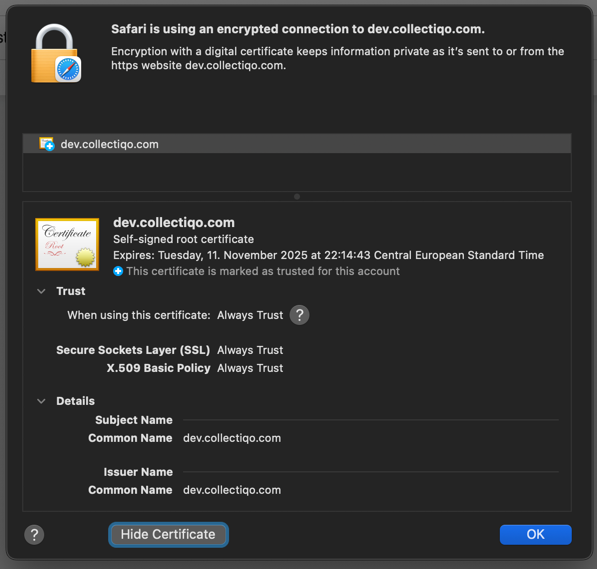
\includegraphics[width=0.5\textwidth]{https_browser}
    \caption{Zertifikat Ansicht in Safari}
    \label{fig:https_browser}
\end{figure}

Diese Schritte sind die Voraussetzung für die Implementierung von SSO, welche im nächsten Semester fortgesetzt werden soll.